\scanpage{51}
% archive sheet number: 50

2.1.84.

\deleted{On place sur \deleted{\unsure{chque}} $K$ deux ensembles de pts, $S'_K$ $S''_{K\unsure{\prime\prime|{}}}$\deleted{\unsure{$''$}} \deleted{\unsure{de}}, de telle façon que}

\inserted{$S'_K$ : sommets rouges \quad $S''_K$ : sommets oranges}

\deleted{\deleted{\unsure{b)}} $\forall\,F$ face de $K$, $\partial F\cap S'$ est un polygone top. d'ordre $2\unsure{n|h}$, et sur chaque arête \inserted{$\alpha$} \deleted{il y} de celui ci il y a un pt de $S''$ et un seul, qui est son milieu si $\alpha$ est contenu}

\deleted{a) $\forall\,S'_K$ \unsure{de} \unsure{tt} \unsure{pt} tous les sommets} \deleted{a) $S'_K\supset S(K)$, $S'_K\supset\unsure{S_2}K\cap L\smallsetminus K\cap S(L)$}

\deleted{a) $S'_K\cap L=K\cap L\smallsetminus(\text{ensemble des pts critiques de $K$ qui sont d'ordre pair})$}

\deleted{b) $S'_K\cap S(K)=S(K)\cap L$}

\deleted{b) \deleted{\unsure{Tout}} Pour toute arête (anc.) $a$ de $K$, on a $a\cap S'_K\ne\varnothing$.} \inserted{\deleted{dans \deleted{une} arête de $K$, et l'unique sommet de $K$ sur $\alpha$ dans le cas inverse.}}

\figure{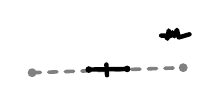
\begin{tikzpicture}[x=0.008cm,y=-0.008cm,line cap=round,line join=round]
\draw[gray,line width=1.3pt,dashed] (0,45)--(240,37);
\draw[line width=1.6pt] (90,40)--(151,39);
\draw[line width=1.6pt] (118,32)--(119,49);
\fill[gray] (0,45) circle [radius=1.6pt];
\fill[gray] (240,37) circle [radius=1.6pt];
\fill[black] (90,40) circle [radius=1.2pt];
\fill[black] (151,39) circle [radius=1.2pt];
\draw[line width=1.6pt] (205,-14)--(212,-14)--(215,-9)--(217,-22)--(220,-13)--(223,-19)--(226,-13)--(230,-23)--(233,-11)--(250,-16);
\end{tikzpicture}}

\figure{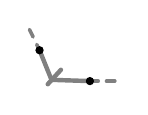
\begin{tikzpicture}[x=0.008cm,y=-0.008cm,line cap=round,line join=round]
\draw[gray,line width=1.3pt,dashed] (0,0)--(16,33);
\draw[gray,line width=1.6pt] (16,33)--(35,80)--(96,82);
\draw[gray,line width=1.6pt] (29,87)--(50,64);
\draw[gray,line width=1.3pt,dashed] (96,82)--(140,82);
\fill[black] (16,33) circle [radius=1.5pt];
\fill[black] (96,82) circle [radius=1.5pt];
\end{tikzpicture}}

\deleted{\unsure{Ex} \uline{NB} a) et b) impliquent que $S'_K\cap S(K)=S(K)\cap L$ i.e. un sommet de $K$ est dans $S'_K$ sss il est dans \unsure{la|L}}

\deleted{c) \deleted{$S'_K\smallsetminus S'_K\cap L$ est réunion de segments, un pour chaque} P\textsubscript{r} un \unsure{tt} pt critique $s$ de $K$, sur l'arête \deleted{arête} \inserted{de} ord \deleted{\unsure{notée $a$}} \inserted{$K$} \deleted{$a$ qui} désignant par $t',t''$ les pts les plus proches de $s$, sur l'arête $a$ de $K$ contenant $s$, parmi les pts de $(a\cap L)\cap\partial a$ \deleted{on dispose sur le segment $[t',t'']$} \inserted{l'intersection $[t',t'']\cap S'_K$ est de cardinal égal à} $\nu(s)$, \deleted{et il y a la}}

\figure{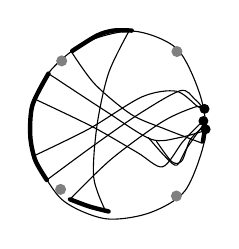
\begin{tikzpicture}[x=0.007cm,y=-0.007cm,line cap=round,line join=round]
\draw[thin] plot[smooth cycle] coordinates {(42,78) (108,23) (196,2) (275,34) (317,118) (326,195) (290,291) (224,332) (144,342) (66,307) (18,229) (9,149)};
\draw[line width=1.6pt] plot[smooth] coordinates {(85,38) (130,10) (160,1) (193,1)};
\draw[line width=1.6pt] plot[smooth] coordinates {(42,79) (13,136) (9,192) (18,236) (39,272)};
\draw[line width=1.6pt] plot[smooth] coordinates {(81,307) (116,320) (151,329)};
\draw[line width=1.6pt] plot[smooth] coordinates {(324,164) (326,177) (322,202)};
\fill[gray] (66,56) circle [radius=2pt];
\fill[gray] (275,39) circle [radius=2pt];
\fill[gray] (64,289) circle [radius=2pt];
\fill[gray] (274,301) circle [radius=2pt];
\draw[thin] plot[smooth] coordinates {(188,2) (151,78) (130,173) (124,267) (145,327)};
\draw[thin] plot[smooth] coordinates {(84,40) (126,98) (192,153) (252,179) (320,205)};
\draw[thin] plot[smooth] coordinates {(42,79) (144,146) (228,198) (280,195) (327,182)};
\draw[thin] plot[smooth] coordinates {(21,127) (123,176) (203,222) (249,248) (286,202) (322,165)};
\draw[thin] plot[smooth] coordinates {(16,228) (116,179) (212,121) (274,111) (313,139) (327,143)};
\draw[thin] plot[smooth] coordinates {(39,272) (119,213) (205,153) (281,110) (307,125) (324,143)};
\draw[thin] plot[smooth] coordinates {(81,307) (156,234) (249,166) (310,139) (325,143)};
\draw[thin] plot[smooth] coordinates {(223,195) (255,231) (275,245) (293,214) (322,173)};
\draw[thin] plot[smooth] coordinates {(238,202) (266,239) (284,237) (299,199) (321,177)};
\fill[black] (325,143) circle [radius=1.8pt];
\fill[black] (323,165) circle [radius=1.8pt];
\fill[black] (327,180) circle [radius=1.8pt];
\end{tikzpicture}}

\figure{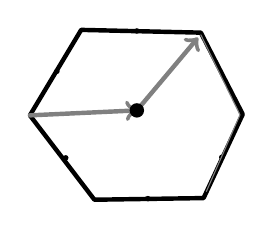
\begin{tikzpicture}[x=0.007cm,y=-0.007cm,line cap=round,line join=round]
\draw[line width=1.6pt] (0,155)--(93,0)--(310,5)--(386,153)--(315,305)--(117,308)--cycle;
\fill[black] (49,75) circle [radius=1pt];
\fill[black] (194,2) circle [radius=1pt];
\fill[black] (348,231) circle [radius=1pt];
\fill[black] (214,306) circle [radius=1pt];
\fill[black] (65,232) circle [radius=1pt];
\draw[gray,line width=1.6pt,->] (0,155)--(194,146);
\draw[gray,line width=1.6pt,->] (194,146)--(305,14);
\fill[black] (194,146) circle [radius=2.6pt];
\draw[gray,thin] (310,9)--(381,154)--(320,293);
\end{tikzpicture}}

\figure{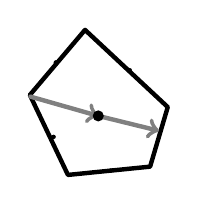
\begin{tikzpicture}[x=0.007cm,y=-0.007cm,line cap=round,line join=round]
\draw[line width=1.6pt] (0,118)--(100,0)--(250,140)--(218,248)--(69,263)--cycle;
\fill[black] (47,59) circle [radius=.8pt];
\fill[black] (181,73) circle [radius=.8pt];
\fill[black] (147,255) circle [radius=.8pt];
\fill[black] (43,194) circle [radius=.8pt];
\draw[gray,line width=1.6pt,->] (1,121)--(124,156);
\draw[gray,line width=1.6pt,->] (124,156)--(234,183);
\fill[black] (124,156) circle [radius=2pt];
\end{tikzpicture}}

\figure{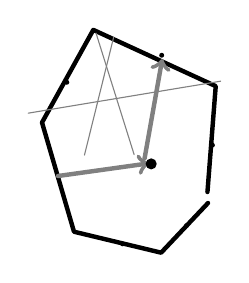
\begin{tikzpicture}[x=0.007cm,y=-0.007cm,line cap=round,line join=round]
\draw[line width=1.6pt] (300,304)--(315,112)--(93,10)--(0,178)--(58,376)--(216,414)--(301,324);
\fill[black] (45,105) circle [radius=.9pt];
\fill[black] (217,56) circle [radius=.9pt];
\fill[black] (309,219) circle [radius=.9pt];
\fill[black] (262,365) circle [radius=.9pt];
\fill[black] (146,398) circle [radius=.9pt];
\fill[black] (30,276) circle [radius=.9pt];
\draw[gray,line width=1.6pt,->] (29,275)--(194,252);
\draw[gray,line width=1.6pt,->] (186,243)--(218,63);
\fill[black] (198,253) circle [radius=2pt];
\draw[gray,thin] (-25,161)--(324,103);
\draw[gray,thin] (130,23)--(77,237);
\draw[gray,thin] (98,16)--(167,236);
\end{tikzpicture}}

\figure{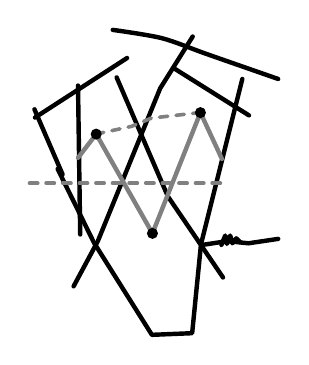
\begin{tikzpicture}[x=0.007cm,y=-0.007cm,line cap=round,line join=round]
\draw[line width=1.6pt] (9,182)--(60,300);
\draw[line width=1.6pt] (51,290)--(117,424)--(222,591)--(295,588)--(311,427)--(386,127);
\draw[line width=1.6pt] (80,503)--(124,421)--(237,144)--(296,50);
\draw[line width=1.6pt] (158,124)--(251,340)--(351,487);
\draw[line width=1.6pt] (88,139)--(92,409);
\draw[line width=1.6pt] (10,197)--(177,89);
\draw[line width=1.6pt] plot[smooth] coordinates {(151,38) (240,53) (322,82) (451,127)};
\draw[line width=1.6pt] (261,107)--(398,193);
\draw[line width=1.6pt] (313,428)--(359,421)--(397,425)--(451,417);
\draw[gray,line width=1.6pt] (88,270)--(121,227)--(223,407)--(310,188)--(349,272);
\draw[gray,line width=1.3pt,dashed] (120,227)--(185,213)--(221,198)--(309,188);
\draw[gray,line width=1.3pt,dashed] (0,316)--(355,316);
\fill[black] (121,227) circle [radius=2pt];
\fill[black] (223,407) circle [radius=2pt];
\fill[black] (310,188) circle [radius=2pt];
\draw[line width=1.6pt] (348,428)--(355,411)--(358,426)--(364,411)--(368,425)--(375,416)--(382,423);
\end{tikzpicture}}

\figure{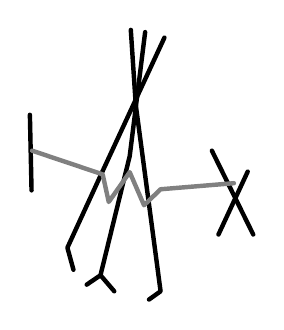
\begin{tikzpicture}[x=0.007cm,y=-0.007cm,line cap=round,line join=round]
\draw[line width=1.6pt] (0,140)--(3,277);
\draw[line width=1.6pt] (79,421)--(68,381)--(131,244)--(244,0);
\draw[line width=1.6pt] (103,448)--(128,431)--(181,215)--(209,-10);
\draw[line width=1.6pt] (129,432)--(153,460);
\draw[line width=1.6pt] (183,-14)--(192,122)--(237,460)--(216,475);
\draw[line width=1.6pt] (330,205)--(405,357);
\draw[line width=1.6pt] (342,357)--(395,243);
\draw[gray,line width=1.6pt] (4,205)--(132,248)--(143,298)--(181,244)--(207,304)--(237,275)--(370,264);
\end{tikzpicture}}
